\documentclass{rentai-chugoku}
%%%%%%%%%%%%%%%%%%%%%%%%%%%%%%%%%%%%%%%%%%%%%%%%%
\usepackage{amsmath,amssymb,amsfonts}
\usepackage{algorithmic}
\usepackage{cite}
\usepackage[dvipdfmx]{graphicx}
\usepackage[dvipdfmx]{xcolor}
\usepackage{newtxtext,newtxmath}
\usepackage{textcomp}
\usepackage{url}
\usepackage{xcolor}
\usepackage{wrapfig}
%%%%%%%%%%%%%%%%%%%%%%%%%%%%%%%%%%%%%%%%%%%%%%%%%
\title{
多数目的最適化における超円錐体積に基づく選択指標の有効性の検討
}

\author{
師田 裕二郎$^*$,Md Kawsar Khan,大木 誠\\
 (鳥取大学)
}

\etitle{
A Consideration on Selection Criterion based on Volume of Hypercone for Many-objective Optimization
}

\eauthor{
Yujiro Morota, Md. Kawsar Khan and Makoto Ohki
(Tottori University)
}

\begin{document}
\setlength\kanjiskip{0.4pt plus 2pt minus 0.4pt}
\maketitle
%%%%%%%%%%%%%%%%%%%%%%%%%%%%%%%%%%%%%%%%%%%%%%%%%%%%%%%%%%%%%%%%%
\section{はじめに}
複数の評価指標(すなわち目的)が数値化されており、協調もしくは競合の関係にあり、それらを最大化もしくは最小化するように対象を変更するような問題を多目的最適化問題(MOP)と呼ぶ。
一般に目的数が多い場合、ほぼ全ての探索点どうしが非支配的になりやすいため、点どうしの優劣が判定できず、最適化を推し進めることが難しい。
このことから、$4$個以上の目的を有する問題を多数目的最適化問題(MaOP)と呼び区別される。
MaOP研究における近年の最適化アルゴリズムは、大きく支配関係に基づく手法、分割に基づく手法、その他の参照点に基づく手法に分類できる。
NSGAは、非支配選択と追加選択の2段階の選択戦略によって、収束的選択圧および多様的選択圧を実現している。
これに対し、MOEA/Dでは、目的空間に一様に分布した参照点を利用して、多数の目的をスカラー化することで、多数の参照点の方向に向かう選択圧を実現している。
これら意外にも、各目的に特化した極端解を保持するための単一エリート・アーカイブ集合や参照点に最も近い点を保持する一様アーカイブ集合などを利用する手法や、特定の探索点と底点の座標との角度を利用した支配関係の緩和・強化を行う手法などもある。
これらのうち、参照点集合を利用したNSGA-IIIやスカラー化関数を改良したMOEA/D等がMaOPに対して有力であると考えられる。

しかし、それらの手法は多様的選択圧を実現するために、当然ながら多数の参照点を必要とし、それらをどのように生成するかという問題と、参照点と探索点の全ての組合せの距離や角度などのメトリックを求める必要があるなど、計算コストが膨大であるという問題を常に抱えている。
本研究では、参照点集合を必要とせず、多様的選択圧を実現可能な選択指標として、探索点が構成する超円錐の体積を利用する手法を提案する。
提案手法をNSGAの追加選択およびMOEA/Dに適用し、その有効性を検証する。



%%%%%%%%%%%%%%%%%%%%%%%%%%%%%%%%%%%%%%%%%%%%%%%%%%%%%%%%%%%%%%%%%
\section{多数目的最適化における選択指標}

本研究で扱う最適化問題を次式のように定義する。
\begin{equation}
\left\{
\begin{array}{ll}
\max.& {\bf f}({\bf x}) = \left[ f_1({\bf x}), \cdots, f_M({\bf x})  \right]^T
\\
{\rm s.t.}& {\bf x} \in {\bf D}
\end{array}
\right.
\end{equation}
このような多数目的最適化問題をとくためのアルゴリズムでは、探索点間の優劣を決定するための選択指標が重要である。
従来研究において用いられている選択指標を以下に示す。





\paragraph{支配関係}
多数目的最適化問題を解く際に、探索点間における優劣を決定する必要があるが、この優劣という言葉は支配と言い換えることができる。
2点$x$,$y$が存在すると仮定すると、$x$が$y$よりも優秀な評価を持つ場合において$x$は$y$を支配するという。
この探索点間の優劣(支配)の判断の基準となるものを支配関係と呼ぶ。
従来の多目的最適化において、パレート支配と呼ばれる手法が支配関係としてたびたび用いられており、NSGA-IIやNSGA-IIIにおいては、各世代において探索点どうしの支配関係に基づいてランク付けする。
多目的最適化のゴールは、制約条件を満たす他のどの解と比べても全ての目的値において劣っていないような解を求めることである。
多目的最適化では、このような解をパレート最適解と呼び、このような解の集合をパレート最適解集合と呼ぶ。
$x$が$y$に支配される状況を次のように定式化できる。
\begin{equation}
\forall j \in {M}:{\bf f}_j({\bf y}) \geqq {\bf f}_j({\bf x}) \land \exists j \in M:{\bf f}_j({\bf y}) > {\bf f}_j({\bf x})
\end{equation}



\paragraph{混雑距離}
\begin{figure}[b]
\begin{center}
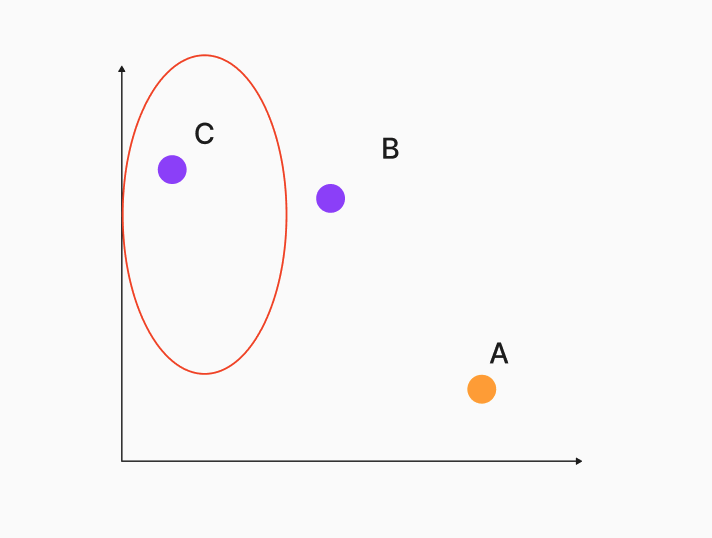
\includegraphics[width=0.5\textwidth]{noSelected.png}
\end{center}
\label{noSelected}
\caption{混雑距離を多目的最適化に使用することによって発生する弊害}
\end{figure}
混雑距離とはある個体の周りにある個体の密度を評価するための手法であり、各目的関数軸において隣り合う個体間の距離を足し合わせたものである。
混雑距離は多目的最適化アルゴリズムの選択戦略において、なるべく解の多様性を維持する目的で用いられる。多目的空間$|M|$におけるフロント集合$F_j$の点${\bf f}({\bf x}_{j}^i)$の混雑距離の定義式を以下に示す。
\begin{equation}
    {\bf f}({\bf x}_{j}^i)=\left[\prod_{m=1}^{|M|} \left|{\bf f}_m\left({\bf x}_{j-1}^i\right)-{\bf f}_m\left({\bf x}_{j+1}^i\right)\right|\right]
\end{equation}
図2は混雑距離によってNSGA等のアルゴリズムで探索点の選択を行う際に赤線で囲まれるエリアが選択されにくくなることを示す。
混雑距離の定義に従い点Aが選択されたと仮定すると、点Cは優先して選択されない。
この時Cの近辺のエリアにあるような個体は同様に選択されなくなるので最適解の集合に点Cのエリアのものが入らなくなってしまう。
このようにして混雑距離を多目的最適化に用いた際に多様性が失われることがある。


\paragraph{重み付き和によるスカラー化}
MOEA/Dは初めに初期個体をスカラー化するするが、そのスカラー化に用いられる手法の一つがこの重み付き和スカラー化である。

次式のように多数の目的を単純にスカラー化する。
\begin{equation}
\begin{array}{ll}
g^{ws}({\bf x}; \lambda)=\lambda \cdot {\bf f}({\bf x})=\sum_{i=1}^{M} \lambda \cdot {\bf f({\bf x})}
\\
\lambda=\left[ \lambda_1, \cdots, \lambda_M \right]^T
\end{array}
\end{equation}
この単一の目的関数$g^{ws}\left({\bf x}; \lambda \right)$を最大化する問題を得る。

\begin{equation}
\left\{
\begin{array}{ll}
\max.& g^{ws}({\bf x}; \lambda)
\\
{\rm s.t.}& {\bf x} \in {\bf D}
\end{array}
\right.
\end{equation}
\paragraph{PBIスカラー化}
MOEA/Dは初めに初期個体をスカラー化するするが、そのスカラー化に用いられる手法の一つがこのPBIスカラー化である。
次式のように多数の目的を単純にスカラー化する。
\begin{equation}
g^{bi/p}\left({\bf x};\lambda,z^* \right)=d_1+\theta d_2
\end{equation}
ただし、
\begin{equation}
\left\{
\begin{array}{ll}
d_1=\frac{\left\|\left(z^*-{\bf f}(\bf x)\right)^t\right\|}{\|\lambda\|}
\\
d_2=||{\bf f}({\bf x})-(z^*-d_1\lambda)||
        % {\rm s.t.}& {\bf x} \in {\bf D}
\end{array}
\right.
\end{equation}
この単一の目的関数$g^{bi/p}(\left[{\bf x};\lambda,z^*\right])$を最小化する問題を得る。
\begin{equation}
\left\{
\begin{array}{ll}
\min.& g^{bi/p}\left({\bf x};\lambda,z^*\right)
\\
{\rm s.t.}& {\bf x} \in {\bf D}
\end{array}
\right.
\end{equation}

\paragraph{Tchebyshevスカラー化}
MOEA/Dは初めに初期個体をスカラー化するするが、そのスカラー化に用いられる手法の一つがこのTchebyshevスカラー化である。
次式のように多数の目的を単純にスカラー化する
\begin{equation}
\begin{array}{ll}
g^{ws}({\bf x}; \lambda,z^*)=\max_{i \in M} {{\lambda \cdot |{\bf f}_i({\bf x})-z_i^*|}}
\\
z^* = \left[ z^*_1, \cdots, z^*_m \right]^T
\\
z_i = \max\{ {\bf f}_i({\bf x})|{\bf x} \in {\bf D} \}  
\end{array}
\end{equation}
この単一の目的関数$g({\bf x}; \lambda,z^*)$を最小化する問題を得る。
\begin{equation}
\left\{
\begin{array}{ll}
\min.& g^{ws\left({\bf x}; \lambda , z^*\right)}
\\
{\rm s.t.}& {\bf x} \in {\bf D}
\end{array}
\right.
\end{equation}

\paragraph{角度支配}
以下は最小化問題を想定した際の角度支配の定義である。
\begin{figure}[b]
\begin{center}
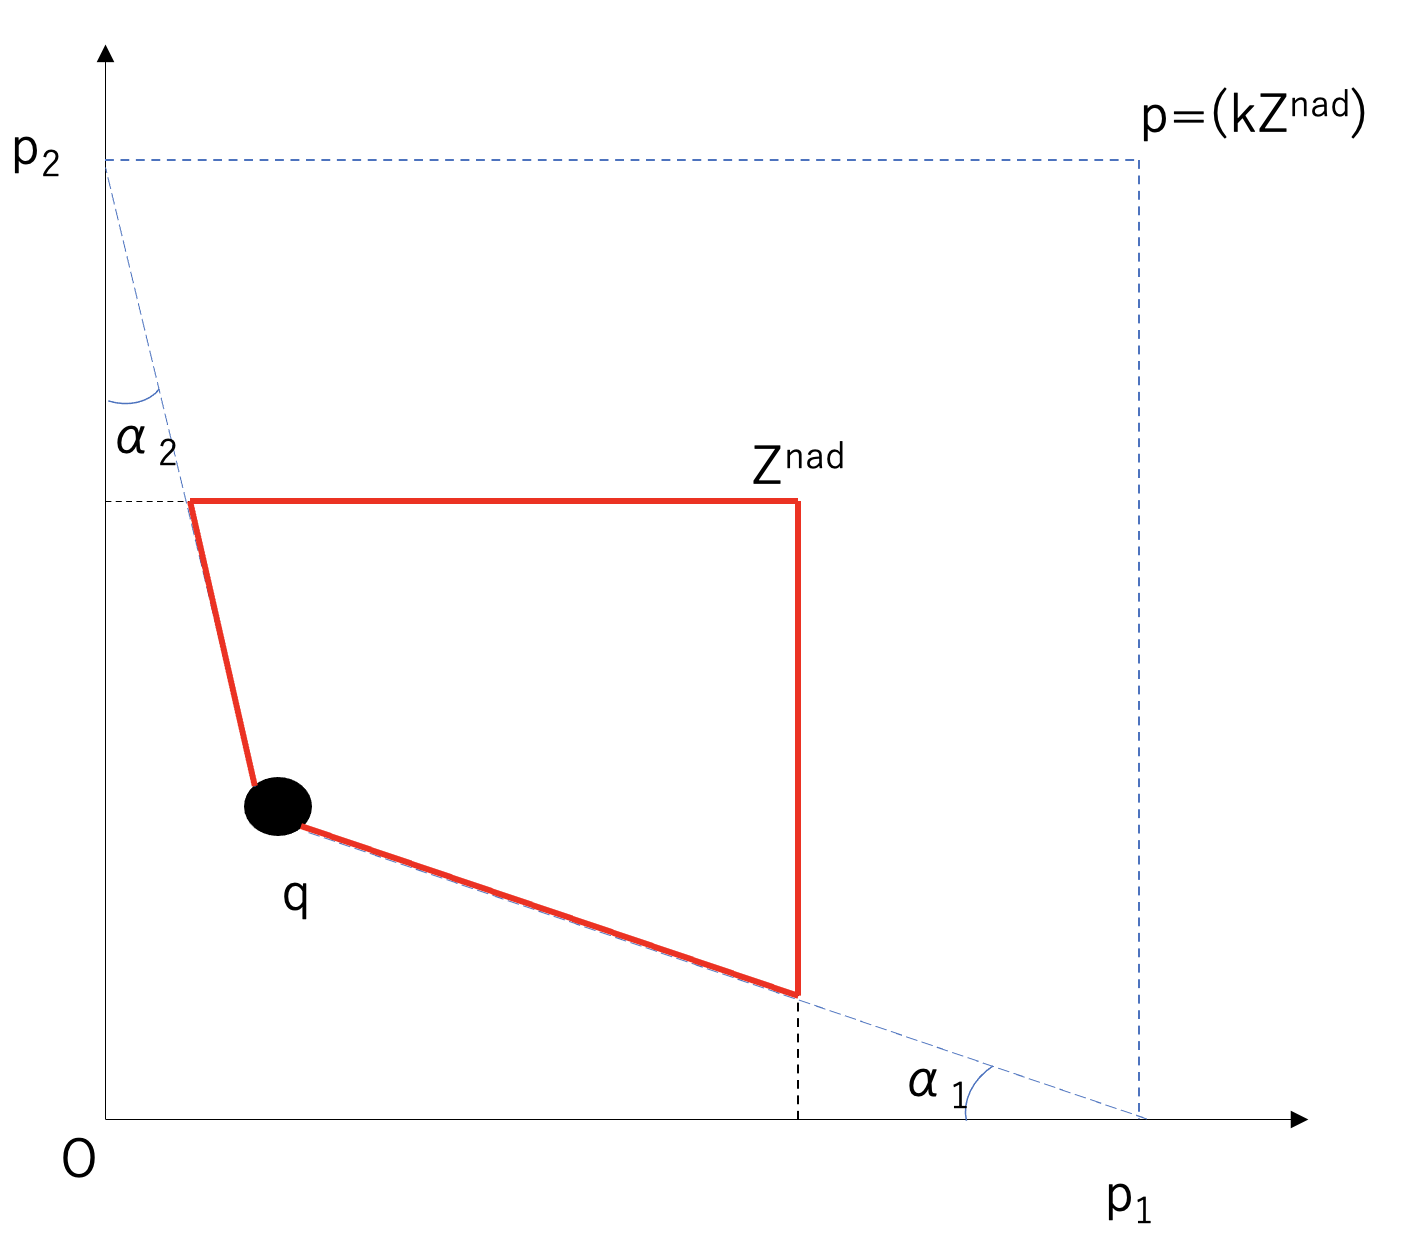
\includegraphics[width=0.5\textwidth]{angle-dominance.png}
\end{center}
\label{angle-dominance}
\caption{2目的の最小化問題におけり解Pの支配領域}
\end{figure}
まず、各目的において最悪の評価値を要素にもつ点$z^{nad}$を求める。
今回は最小化問題であるため$z^{nad}$は各目的における最大値を要素にもつ点となる。
$i$番目の目的関数における最悪の評価値$z^{nad}_i$は以下のようになる。
\begin{equation}
z^{nad}_{i} = \max^{n}_{j=1} f_i(x_j)
\end{equation}
$z^{nad}_i$を要素にもつ点$z^{nad}$は以下のようになる。
\begin{equation}
z^{nad}=\left[z^{nad}_1,z^{nad}_2 \cdots ,z^{nad}_i\right]
\end{equation}
その点を$k$倍した点を$p$とする。
\begin{equation}
p=kz^{nad}=\left[kz^{nad}_1,kz^{nad}_2 \cdots ,kz^{nad}_i\right]
\end{equation}
% $i$番目の目的関数における$kz^{nad}$を$p_i$とする。
% \begin{equation}
% p_i=kz^{nad}_{i} 
% \end{equation}
$i$目的番目における点$p_i$を以下のように定義する。
\begin{equation}
p_i=\left(0,\cdots,kz^{nad},\cdots,0\right)
\end{equation}


そして解$q$、点$p_{i}$、点$p$で構成される角度$\alpha$を次のように定義する。
\begin{equation}
\alpha_i=\arccos{\frac{\vec{p_{i}o} \vec{p_{i}q}}{|\vec{p_{i}o}| |\vec{p_{i}q}|}}
\end{equation}
この$\alpha_i$を要素にもつ角度ベクトルを定義し、解$q$がこの角度ベクトルを保持する。
\begin{equation}
angle_{q}=\left(\alpha_1,\alpha_2,\cdots \alpha_i \right)
\end{equation}
% 2点$x$、$y$が存在すると仮定するとき、以下の条件が成立すれば、$x$が$y$を支配することになる。
2点$x$、$y$が存在すると仮定すると、解$x$、$y$に以下の角度ベクトルを割り振ることができる。
\begin{equation}
angle_{x}=\left(\alpha^{x}_1,\alpha^{x}_2,\cdots \alpha^{x}_i \right)
\end{equation}
図2の赤線で囲まれる部分が解$q$が支配する範囲となる。
\begin{equation}
angle_{y}=\left(\alpha^{y}_1,\alpha^{y}_2,\cdots \alpha^{y}_i \right)
\end{equation}
以下の条件が成立すれば、$x$が$y$を支配することになる。
\begin{equation}
\forall i \in {\{1,2, \cdots,M}\}:\alpha^{x}_{i}< \alpha^{y}_{i}
\end{equation}


%%%%%%%%%%%%%%%%%%%%%%%%%%%%%%%%%%%%%%%%%%%%%%%%%%%%%%%%%%%%%%%%%
\section{超円錐体積に基づく選択指標}

\begin{figure}[b]
\begin{center}
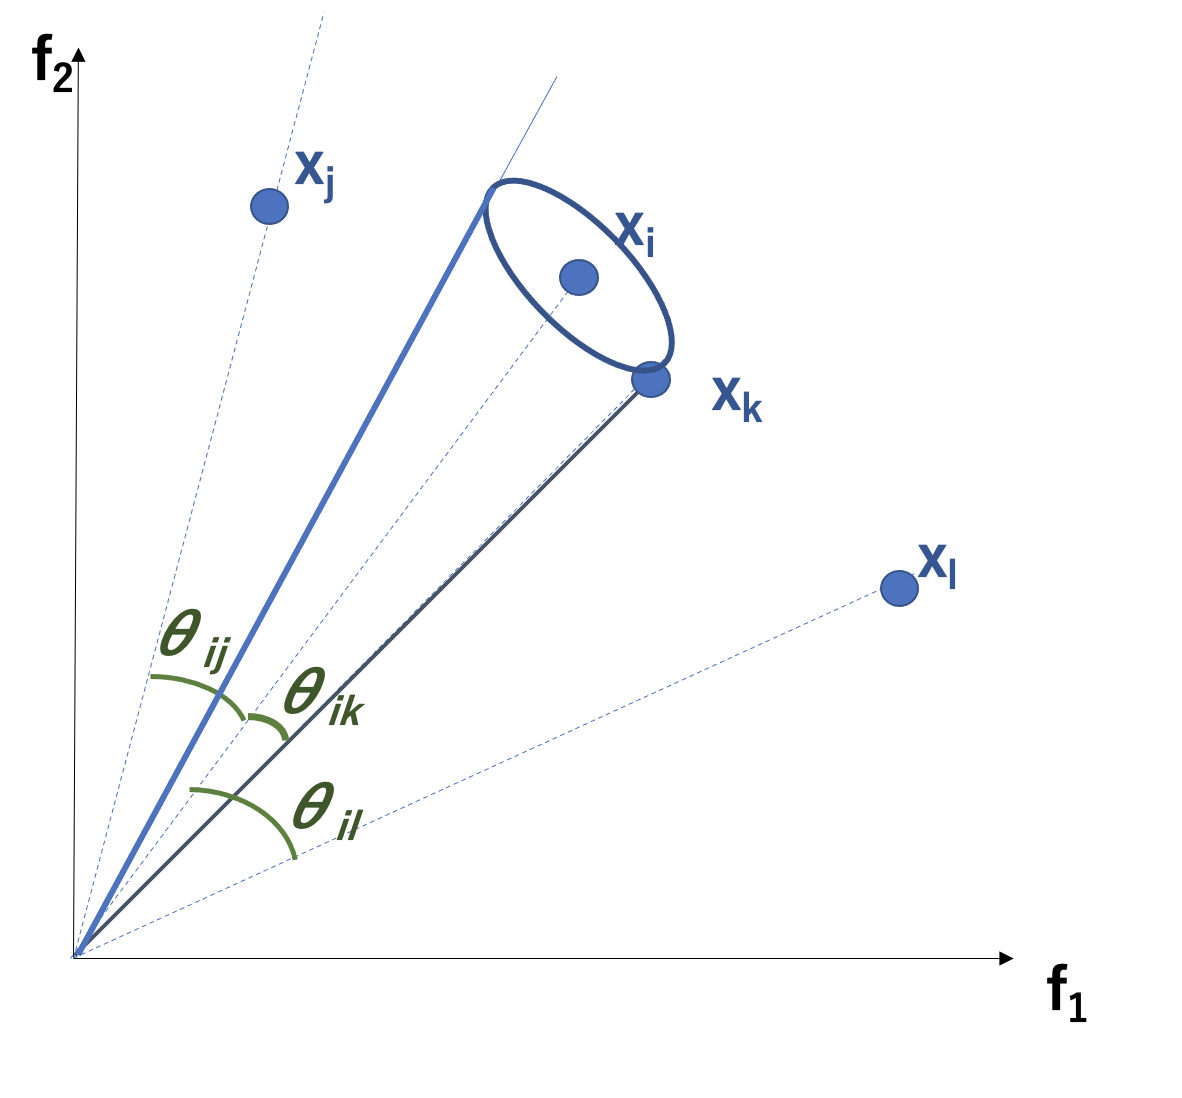
\includegraphics[width=0.3\textwidth]{hv.png}
\end{center}
\label{hypercone}
\caption{
探索点間の位置関係に基づく超円錐の定義
}
\end{figure}
ある最適化世代における探索点集合${\bf X}$の例を図\ref{hypercone}に示す。
探索点${\bf f}\left( {\bf x}_i \right)$に注目し、点${\bf f}\left( {\bf x}_i \right)$と他の全ての点${\bf f}\left( {\bf x}_j \right)$との相対角は次式を満たす。
\begin{equation}
\cos \theta_{i,j} = \cos \theta_{j,i} = 
\frac{ {\bf f}\left( {\bf x}_i \right) }{\left\| {\bf f}\left( {\bf x}_i \right) \right\|}
\cdot
\frac{ {\bf f}\left( {\bf x}_j \right) }{\left\| {\bf f}\left( {\bf x}_j \right) \right\|}
\label{cos}
\end{equation}
この角$\theta_{i,j}$を最小とする他点${\bf f}\left( {\bf x}_k \right)$を特定するためには、式\ref{cos}を最大とする点を求めればよい。
このようにして得られた角$\theta_{i,k}$を用いて、点${\bf f}\left( {\bf x}_i \right)$と点${\bf f}\left( {\bf x}_k \right)$の距離を次式のように定義する。
\begin{equation}
r_{i,k} = \frac{ \left\| {\bf f}\left( {\bf x}_i \right) \right\| }
{ \sin \theta_{i,k}}
%= \left\| {\bf f}\left( {\bf x}_i \right) \right\| {\rm cosec} \theta_{i,k}
= \frac{\sqrt{ \left\| {\bf f}\left( {\bf x}_i \right) \right\|^3\cdot \left\| {\bf f}\left( {\bf x}_k \right) \right\| }}
{\sqrt{ \left\| {\bf f}\left( {\bf x}_i \right) \right\|\cdot \left\| {\bf f}\left( {\bf x}_k \right) \right\| - {\bf f}\left( {\bf x}_i \right)\cdot {\bf f}\left( {\bf x}_k \right)}}
\end{equation}
この$r_{i,k}$を半径とし、中心を点${\bf f}\left( {\bf x}_i \right)$とする円をの面積を$S(r_{i,k})$とすると、図の円錐の超体積$V_i$は次式で与えられる。
\begin{equation}
V_i = \frac{1}{M} \left\| {\bf f}\left( {\bf x}_i \right) \right\| \cdot S(r_{i,k})
\end{equation}
ここで、底面積$S(r_{i,k})$は$M$次元空間における円の面積であるから、半径を$r_{i,k}$とする$M-1$次元の超球の体積として与えられる。
\begin{eqnarray}
S(r_{i,k}) 
= \frac{ \displaystyle\pi^\frac{M-1}{2}\cdot r_{i,k}^{M-1} }{ \displaystyle\Gamma\left( \frac{M+1}{2} \right) }
\hspace{30mm}\\
= \left\{
\begin{array}{ll}
\displaystyle\frac{ \displaystyle\pi^{\frac{M-1}{2}} }{ \displaystyle\left( \frac{M-1}{2} \right)! } r_{i,k}^{M-1} & M:{\rm odd}\\
\\
\displaystyle\frac{\displaystyle2^{\frac{M}{2}}\cdot \displaystyle\pi^{\frac{M-2}{2}}}{\left( M-1 \right)!!} r_{i,k}^{M-1} & M:{\rm even}
\end{array}
\right.
\end{eqnarray}
従って、超円錐の体積$V_i$は次式によって与えられる。
\begin{equation}
V_i = 
\left\{
\begin{array}{ll}
\displaystyle\frac{ \displaystyle\pi^{\frac{M-1}{2}} }{ M\cdot\displaystyle\left( \frac{M-1}{2} \right)! } r_{i,k}^{M-1} \cdot\left\| {\bf f}\left( {\bf x}_i \right) \right\| & M:{\rm odd}\\
\\
\displaystyle\frac{\displaystyle2^{\frac{M}{2}}\cdot \displaystyle\pi^{\frac{M-2}{2}}}{M\cdot\left( M-1 \right)!!} r_{i,k}^{M-1} \cdot\left\| {\bf f}\left( {\bf x}_i \right) \right\| & M:{\rm even}
\end{array}
\right.
\end{equation}


%%%%%%%%%%%%%%%%%%%%%%%%%%%%%%%%%%%%%%%%%%%%%%%%%%%%%%%%%%%%%%%%%
\section{NSGAおよびMOEA/Dに対する提案手法の適用}
\paragraph{NSGAに対する提案手法の適用}
従来のNSGAは追加選択の過程において混雑距離大きいものを優先的に選択するようになっており、混雑距離が小さい個体は全く選択されなくなってしまう。
これが多様性を失うことにつながっていると考えられる。そこでNSGAの追加選択の過程に提案手法を用いることで、多様性が下がることを防ぐことができる。
以下にNSGAに提案手法を組み込んだ際の流れを示す。
また、図3にNSGAに提案手法を組み込んだ際の流れを図示した。
\begin{enumerate}
\item 非支配ソーティング\\
サイズ$2N$の第$ t $世代の個体集合$R_t$に対して非支配ソーティングを行い、フロント集合$F_1,F_2,\cdots $を得る。
\item ランキング上位半分以上のランク選択\\
親個体集合のサイズ$ N $に満たないまでのフロント集合を得る。
\\ $F_1+F_2+ \cdots+ F_s \geqq{N}$を満たす最初のsを求める(sはランク)
\item 追加選択\\
親個体集合の半分のサイズNを超えるフロント集合について、提案手法である超円錐堆積に基づいたランキング選択を行い上位$ N - \sum_{k=1}^{s-1}F_k $個の個体を得る。\\
この時、提案手法に基づいて計算された体積が、最大化問題であれば、体積が大きものから順に良い個体となり、最小化問題であればより体積が小さい個体を選択していくことになる。
\\ $s-1$ランクまでの個体集合にこれらを加えてサイズNの個体集合を生成する。
\item 繰り返し\\ 
$1$から$3$を繰り返す。
\end{enumerate}

\begin{figure}[h]
\begin{center}
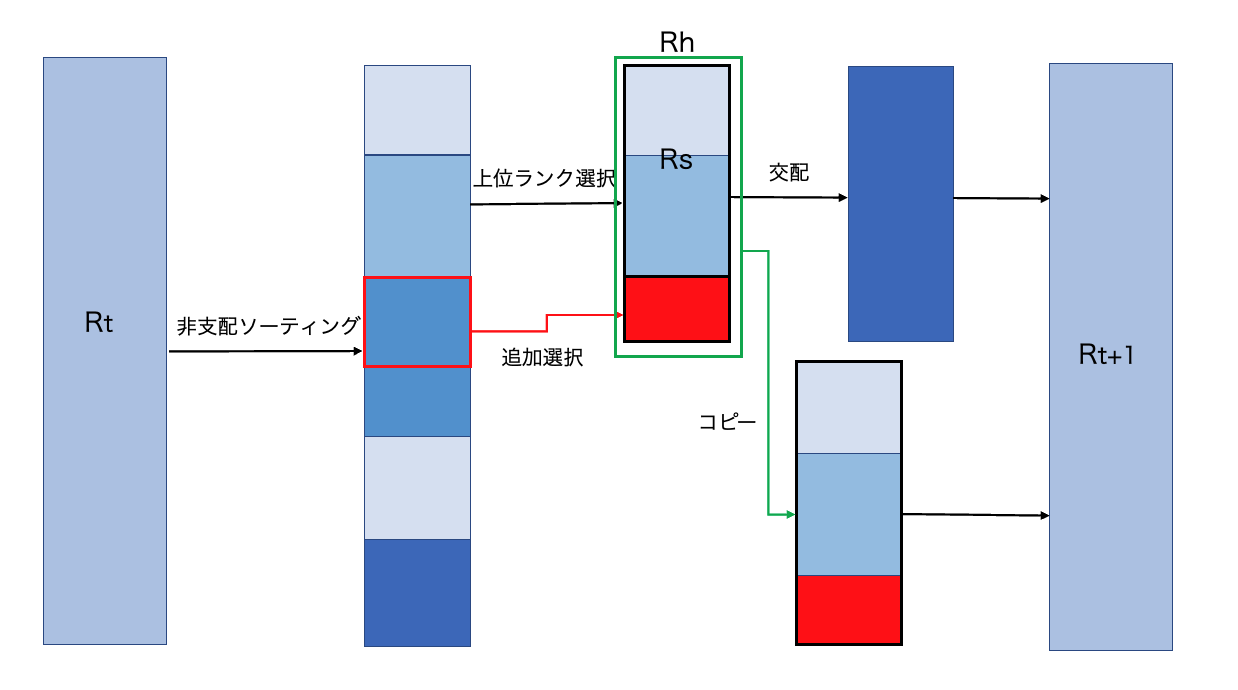
\includegraphics[width=0.5\textwidth]{NSGA2.png}
\end{center}
\label{NSGA}
\caption{
提案手法を組み込んだNSGAの流れ
}
\end{figure}
\paragraph{MOEA/Dに対する提案手法の適用}
\begin{figure}[h]
\begin{center}
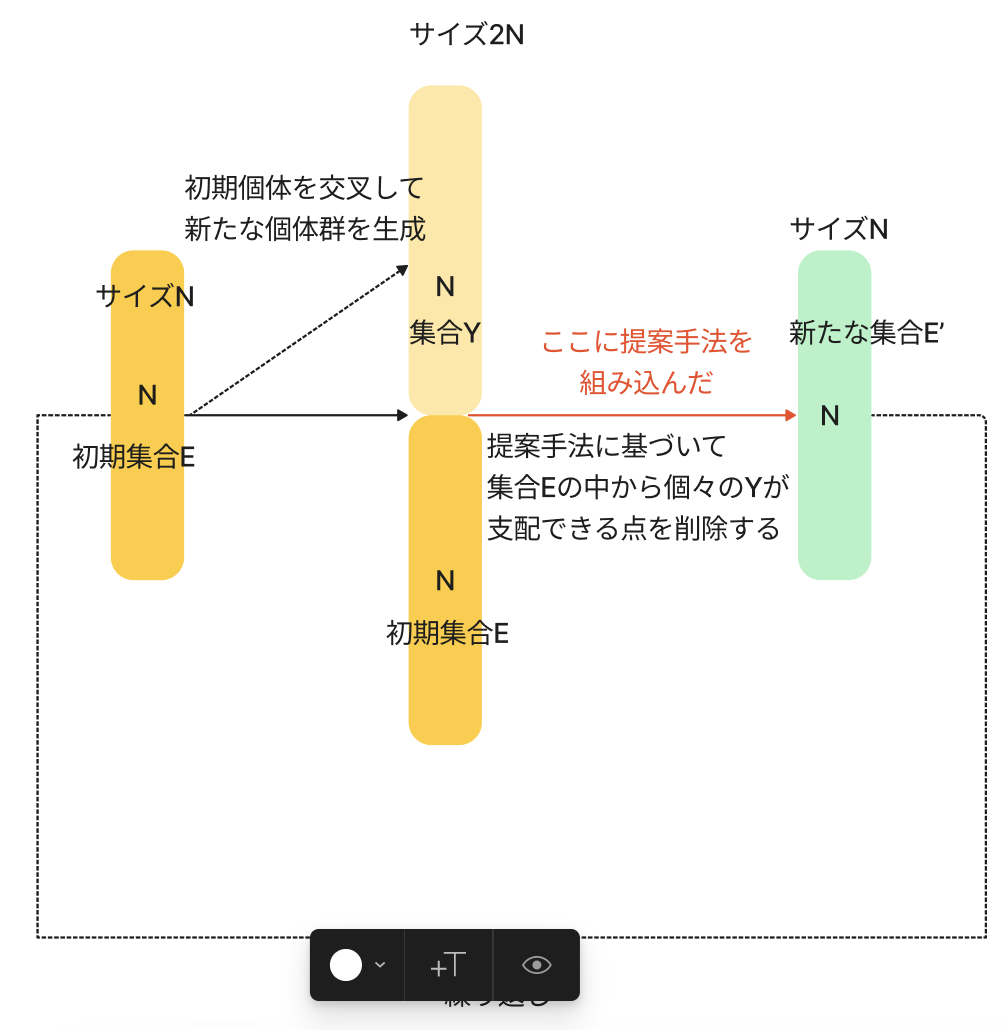
\includegraphics[width=0.5\textwidth]{MOEAD2.png}
\end{center}
\label{MOEA/D}
\caption{提案手法を組み込んだMOEA/Dの流れ}
\end{figure}
従来のMOEA/Dは参照点を必要とするため、計算量が多くなってしまうという問題があるが、本提案手法を組み込んだMOEA/Dは参照点を必要とせず、単純なスカラーで各々のデータの優劣を判定することができる。
そのため計算量が減る可能性がある。
また、上記のNSGAと同様に混雑距離の大きい個体のみを選択することによって多様性が失われるという問題があったが、本提案手法を組み込むことで、多様性が失われることを防ぐことができる。
以下にMOEA/Dに提案手法を組み込んだ際の流れを示す。
また、図4に従来のMOEA/Dに提案手法を組み込んだ際の流れを図示した。
\begin{enumerate}
\item 初期個体の生成\\
初期個体の生成をし$E$とする。
\item 交叉\\
交叉、突然変異を行って子個体を生成し、この個体群を$y$とする。
この時親個体の中からユークリッド距離が最も近い個体を選択し、交叉する。
\item 探索点の更新\\
交叉して生成した個体群$y$の中から1点ずつ取り出し、提案手法を用いて、$y$、$E$の個体の超円錐の体積を計算して、最小化の場合$E$の中から各々の$y$の点よりも超円錐の体積が大きいものを全て削除、最大化の場合超円錐の体積が小さいものを削除する。
\item 繰り返し\\
$1$から$4$を繰り返す。
\end{enumerate}


% %%%%%%%%%%%%%%%%%%%%%%%%%%%%%%%%%%%%%%%%%%%%%%%%%%%%%%%%%%%%%%%%%
% \section{ベンチマークによる有効性の検証}



% %%%%%%%%%%%%%%%%%%%%%%%%%%%%%%%%%%%%%%%%%%%%%%%%%%%%%%%%%%%%%%%%%
% \section{おわりに}


\bibliographystyle{IEEEtran}
\bibliography{references} 

\end{document}
